%!TEX root = "../../DA_GUI.tex"
%	########################################################
% 				Allgemeiner Teil (Theorie)
%	########################################################


%	--------------------------------------------------------
% 	Aufbau der Benutzeroberfläche
%	--------------------------------------------------------


\chapter{Das Hauptfenster von C Compact}
\label{sec:gui-main}
Zu diesem Bereich zählen alle Elemente des Hauptfensters. Der grundlegende Aufbau wurde bereits vor dem Projektstart entworfen und in unserem Praktikum im Sommer 2014 implementiert. Vom Herbst 2014 bis Ende Januar 2015 wurde der Aufbau und die Bedienung dieser Oberfläche erweitert und verbessert. Eine besondere Hilfestellung dabei waren die Versuche mit SchülerInnen der ersten und zweiten Klassen, die an unseren Versuchen teilgenommen haben (siehe Kapitel \ref{sec:sci-trial-intro}).

\section{Basispanel des Hauptfensters}
\label{sec:gui-main-1}
Die Entwicklungsumgebung selbst ist in zwei Hälften geteilt (siehe Abbildung \ref{fig:gui-main-1}). Im linken Teil befinden sich die Textfelder für den Quelltext und für die Ein- und Ausgabe des CMM-Programmes. Im rechten Teil befinden sich Registerkarten mit unterschiedlichen Aktionsfeldern.

Die beiden Teile sind durch einen Balken getrennt, der mit der Maus verschoben werden kann.% Diese Funktionen wurden mit dem Swing-Element JSplitPane\footnote{http://docs.oracle.com/javase/7/docs/api/javax/swing/JSplitPane.html} implementiert.

\begin{figure}[h] 
  \centering
     \includegraphics[width=0.7\textwidth]{./media/images/gui/main/CCompactAlpha1-4-5-guimain.png}
  \caption{Aufbau des Hauptfensters}
  \label{fig:gui-main-1}
\end{figure}

\subsection{Implementierung}
\label{sec:gui-main-impl}
Das Hauptfenster selbst wird von der Klasse \textbf{GUImain} verwaltet. Diese Klasse implementiert, da sie ein Hauptfenster regelt, das Interface \textbf{GUIExecutable}. Zum Starten der Entwicklungsumgebung muss immer ein Objekt dieser Klasse angelegt werden. Im Konstruktor muss eine Referenz auf ein Einstellungsobjekt der Klasse \textbf{GUImainSettings} (siehe Kapitel \ref{sec:guimainsettings}) übergeben werden. In diesem Objekt werden alle Einstellungen des Benutzers gespeichert.

Wenn C Compact ohne Benutzerprofil gestartet werden soll, wird als Parameter \textbf{null} übergeben. In diesem Fall können keine Quests gestartet werden, alle anderen Funktionen wie etwa der Debugger sind aber verfügbar.

\newpage

\begin{lstlisting}[language=JAVA]
	/**
	 * Constructor requires specific configuration for the window (settings)
	 * 
	 * @param settings Configuration object for the main GUI.
	 */
	public GUImain(GUImainSettings settings) {
		this.settings = settings;
	}
\end{lstlisting}

Um das Hauptfenster zu initialisieren und C Compact zu starten, muss danach die Methode \textbf{void start(boolean test)} aufgerufen werden. Diese Methode wurde vom Interface GUIExecutable übernommen. Als Parameter sollte normalerweise \textbf{false} übergeben werden. Wenn \textbf{true} übergeben wird, wird das Fenster gleich nach dem Initialisieren geschlossen. Diese Funktion wird für automatisierte Tests mit ANT verwendet (siehe Kapitel \ref{sec:dev-build-ant}).

\begin{lstlisting}[language=JAVA]
@Override
public void start(boolean test) {
	...
			
	// Fenster initialisieren
	this.jFrame = new JFrame(VERSION);
	this.jFrame.setDefaultCloseOperation(JFrame.DO_NOTHING_ON_CLOSE);
	this.jFrame.getContentPane().setPreferredSize(new Dimension(800, 500));
	this.jFrame.setMinimumSize(new Dimension(600, 400));
		
	...
		
	// Programm beenden, wenn im Testmodus
	if (test)
		System.exit(0);
}
\end{lstlisting}

Außerdem implementiert die Klasse GUImain die Methode \textbf{saveAndDispose()} des Interfaces \textbf{GUIExecutable}. Diese Methode speichert alle Einstellungen und Daten des Benutzers und beendet das Programm.

\begin{lstlisting}[language=JAVA]
	@Override
	public void saveAndDispose() {
		this.getSaveManager().directSave();
		this.getSettings().writeXMLsettings();
		this.dispose();
	}
\end{lstlisting}

\section{Linker Teil der Benutzeroberfläche}
\label{sec:gui-main-left-0}
Zum linken Bereich der Benutzeroberfläche gehören Textfelder für Ein- und Ausgabedaten des CMM-Programmes, das Textfeld für den Sourcecode, sowie ein farbiges Panel, das den aktuellen Zustand der Benutzeroberfläche visualisiert.

Unterschiedliche Elemente oder Gruppen von Bedienelementen werden mit JSplitPanes\footnote{https://docs.oracle.com/javase/tutorial/uiswing/components/splitpane.html} getrennt. Ein JSplitPane enthält immer zwei Swing-Komponenten, die durch einen verschiebbaren Balken getrennt werden. In diesem Fall werden zwei verschachtelte SplitPanes verwendet. Das äußere Panel enthält einerseits das Zustandspanel (siehe Kapitel \ref{sec:gui-main-left-zust}) und das Textfeld für den Sourcecode (siehe Kapitel \ref{sec:gui-main-left-code}), andererseits auch ein zweites SplitPane, das Ein- und Ausgabefeld trennt (Kapitel \ref{sec:gui-main-left-io}).

\subsection{Allgemeine Implementierung}
Der gesamte linke Teil der Benutzeroberfläche ist in der Klasse \textbf{GUIleftPanel} im Package \textbf{at.jku.ssw.cmm.gui} implementiert. Ein Objekt dieser Klasse wird beim Starten von C Compact von \textbf{GUImain} initialisiert.

Für die Kommunikation mit anderen Klassen wurden einige Methoden implementiert, die wichtigsten werden in Tabelle \ref{tab:gui-main-left-methods} aufgelistet.

\def\arraystretch{1.6}
\begin{table}[h!]
\begin{tabular}{|l|p{9cm}|}
\hline
\textbf{Name}&\textbf{Beschreibung}\\
\hline
\hline
public JSplitPane init(...)&Initialisiert diesen Teil der Benutzeroberfläche und gibt eine Referenz auf das Hauptelement zurück\\
\hline
public void setReadyMode()&\multirow{4}{*}{\parbox{9cm}{Ändert den Modus des Zustandpanels, Siehe Kapitel \ref{sec:gui-main-left-zust}}}\\
public void setErrorMode(...)&\\
public void setRunMode()&\\
public void setPauseMode()&\\
\hline
public void lockInput()&\multirow{2}{*}{\parbox{9cm}{Sperrt und ermöglicht Eingabe in eines der Textfelder, Siehe Kapitel \ref{sec:gui-main-left-zust}}}\\
public void unlockInput()&\\
\hline
public void setOrientation(...)&Ändert die Anordnung der Elemente in diesem Teil der Benutzeroberfläche, Siehe Kapitel \ref{sec:gui-main-left-ord} und ...\\
\hline
public void updateFontSize()&Ändert die Schriftgröße in allen Textfeldern\\
\hline
\end{tabular}
\caption{Die wichtigsten Methoden der Klasse \textbf{GUIleftPanel}}
\label{tab:gui-main-left-methods}
\end{table}

Die Textfelder in diesem Teil der Benutzeroberfläche werden mit statischen Methoden initialisiert, die in der Klasse \textbf{InitLeftPanel} im Package \textbf{at.jku.ssw.cmm.gui.init} zu finden sind. Im Folgenden wird bei dem jeweiligen Element erwähnt, in welcher Methode es initialisiert wird.

\pagebreak
\subsection{Anordnung der Elemente}
\label{sec:gui-main-left-ord}

Um C Compact für alle Bildschirmformate optimal anzupassen, sind in den Einstellungen unterschiedliche Optionen zur Anordnung der Elemente im linken Panel zu finden. Die Abbildungen \ref{fig:gui-main-left-o1} bis \ref{fig:gui-main-left-o4} zeigen die möglichen Konfigurationen (siehe auch Kapitel \ref{sec:guimainsettings}).

\begin{figure}[h!]
\centering
	\begin{minipage}{0.45\textwidth}
		\centering
		\includegraphics[width=1.0\textwidth]{./media/images/gui/main/orientations/CCompact-gui-1.png}
		\caption{Classic Vertical}\label{fig:gui-main-left-o1}
	\end{minipage}\hfill
	\begin{minipage}{0.45\textwidth}
		\centering
		\includegraphics[width=1.0\textwidth]{./media/images/gui/main/orientations/CCompact-gui-2.png}
		\caption{Classic Horizontal}\label{fig:gui-main-left-o2}
	\end{minipage}
\end{figure}

\begin{figure}[h!]
\centering
	\begin{minipage}{0.45\textwidth}
		\centering
		\includegraphics[width=1.0\textwidth]{./media/images/gui/main/orientations/CCompact-gui-3.png}
		\caption{Widescreen Central}\label{fig:gui-main-left-o3}
	\end{minipage}\hfill
	\begin{minipage}{0.45\textwidth}
		\centering
		\includegraphics[width=1.0\textwidth]{./media/images/gui/main/orientations/CCompact-gui-4.png}
		\caption{Widescreen Left}\label{fig:gui-main-left-o4}
	\end{minipage}
\end{figure}

Wie in Kapitel \ref{sec:gui-main-left-0} bereits beschrieben wurde, ist der linke Teil der Benutzeroberfläche mit zwei verschachtelten JSplitPanes organisiert. Für einfache Änderungen am Aufbau der Benutzeroberfläche reicht es, die Orientierung eines SplitPanes zu verändern:

\begin{lstlisting}[language=JAVA]
	// Trennbalken ist vertikal
	splitPanel.setOrientation(JSplitPane.VERTICAL_SPLIT);
	
	// Trennbalken ist horizontal
	splitPanel.setOrientation(JSplitPane.HORIZONTAL_SPLIT);
\end{lstlisting}

Mit der Methode \textbf{setOrientation} kann die Anordnung der Elemente im linken Panel verändert werden. Für die dritte mögliche Anordnung (Abbildung \ref{fig:gui-main-left-o3}, \glqq{}Widescreen Central\grqq{}) müssen die Elemente des äußeren Panels allerdings vertauscht werden. Deshalb wird bei jedem Wechsel auf diese Konfiguration die private Methode \glqq{}swap\grqq{} aufgerufen. Wenn als Parameter \textbf{true} übergeben wird, werden die Elemente ausgetauscht, ansonsten werden die Komponenten wieder auf ihre Ausgangsposition geracht.

\begin{lstlisting}[language=JAVA]
	private void swap(boolean def) {
		
		// SplitPane zurücksetzen
		this.outerPane.setTopComponent(null);
		this.outerPane.setBottomComponent(null);
		
		// Elemente neu einfügen (je nach Anordnung)
		if( def ) {
			this.outerPane.setTopComponent(this.jSourceCodeContainer);
			this.outerPane.setBottomComponent(this.innerPane);
		}
		else {
			this.outerPane.setBottomComponent(this.jSourceCodeContainer);
			this.outerPane.setTopComponent(this.innerPane);
		}
	}
\end{lstlisting}

\subsection{Zustandspanel des Debuggers}
\label{sec:gui-main-left-zust}

\begin{figure}[htbp] 
  \centering
     \includegraphics[width=0.7\textwidth]{./media/images/gui/main/CCompact-gui-left-panel.png}
  \caption{Das Zustandspanel während des Debuggens}
  \label{fig:gui-main-left-panel}
\end{figure}

Die Benutzeroberfläche der Entwicklungsumgebung kann vier unterschiedliche Zustände annehmen. Diese Zustände (siehe auch \ref{sec:deb-use}) beziehen sich nur auf die Basisfunktionen der Entwicklungsumgebung und des Debuggers, nicht aber auf den Zustand der zu bearbeitenden Quest.

\subsubsection*{Editormodus}
Der Benutzer kann den Quelltext wie bei einem Texteditor bearbeiten. Auch Eingabedaten für den Debugger können eingegeben werden. Dies ist der Standardzustand, das Zustandspanel ist grau.
\subsubsection*{Fehlermodus} Es ist ein Fehler im Quellcode des Benutzers aufgetreten. Der Fehler wurde entweder im Präprozessor, im Compiler oder im Interpreter erkannt. Das Zustandspanel ist rot und zeigt zusätzliche Informationen zum Fehler, wie etwa die Art des Fehlers und die Zeile, in der der Fehler aufgetreten ist. Im rechten Teil des Hauptfensters wird eine detaillierte Beschreibung des Fehlers gezeigt (siehe Kapitel \ref{sec:deb-error}). In diesem Modus kann der Sourcecode bearbeitet werden, um den Fehler zu beheben.

Der Text im Zustandspanel wird im Fehlermodus aus folgenden Informationen zusammengesetzt:
\begin{enumerate}
\item \textbf{Präfix:} Beschreibender Text am Beginn der Nachricht.
\item \textbf{Dateiname:} Wird nur angegeben, wenn der Fehler in einer externen Datei oder einer Bibliothek aufgetreten ist.
\item \textbf{Zeilennummer:} Die Zeile, in der der Fehler aufgetreten ist.
\item \textbf{Postfix:} Beschreibender Textteil am Ende der Nachricht. Dies ist in manchen Sprachen notwendig, um grammatikalisch vollständige Sätze konstruieren zu können (siehe Beispiel unten).
\end{enumerate}

Die Fehlernachricht wird mit folgendem Code zusammengesetzt. Dieser Teil stammt aus der Funktion \textbf{setErrorMode} in der Klasse \textbf{GUIleftPanel}:

\begin{lstlisting}[language=JAVA]
	// Fehlertext für das Zustandspanel
	this.jStateLabel.setText("<html>! ! ! " +
		// Präfix
		(title[0] == null ? _("error") : title[0]) +
		// Dateiname
		(file == null || file != "main" ? "" : " in file " + file) + " " +
		// Zeilenangabe
		(line >= 0 ? _("in line") + " " + (int)objLine[1] : "") +
		// Postfix
		(title[1] == null ? "" : " " + title[1]) +
	" ! ! !</html>");
\end{lstlisting}

\textbf{Beispiel:}
\[
\underbrace{\text{Semikolon}}_{\text{Präfix}} \underbrace{\text{in der Datei stdio.h}}_{\text{Datei}} \underbrace{\text{in Zeile 15}}_{\text{Zeilenangabe}} \underbrace{\text{(oder vorher) vergessen}}_{\text{Postfix}}
\]

Präfix und Postfix können zu Beginn der Fehlerbeschreibungsdatei definiert werden. Für jeden bekannten Fehler gibt es ein HTLM-Dokument, das einen entsprechenden Beschreibungstext enthält. Diese Fehlerdateien sind im Ordner \textbf{error} im C Compact Programmordner zu finden (siehe auch Kapitel \ref{sec:deb-error}).

\begin{lstlisting}[language=HTML]
<head>
	<prefix>Semikolon</prefix>
	<postfix>(oder vorher) vergessen</postfix>
</head>
\end{lstlisting}

\subsubsection*{Schritt für Schritt debuggen} Dies ist einer der beiden möglichen Modi des Debuggers. In diesem Fall wird das Programm so ausgeführt, dass der Benutzer jeden Schritt des Interpreters selbst initiieren muss (mit dem \glqq{}Nächster Schritt\grqq{}-Button oder die Taste F6). Das Bearbeiten des Sourcecode ist nicht möglich. Das Zustandspanel ist gelb.

\subsubsection*{Austomatisches debuggen} In diesem Modus spring der Debugger  in gewissen Zeitabständen automatisch weiter. Auch hier ist das Bearbeiten des Quelltexts nicht möglich. Das Zustandspanel ist grün.

Das Zustandspanel wird in der Methode \textbf{init()} der Klasse \textbf{GUIleftPanel} initialisiert.

\subsection{Textfeld für den Sourcecode}
\label{sec:gui-main-left-code}
Das Feld für den Quellcode wurde als \textbf{RSyntaxTextArea}\footnote{http://bobbylight.github.io/RSyntaxTextArea/} implementiert. Dieses Projekt wurde von Robert Futrell veröffentlicht und steht unter einer modifizierten BSD-Lizenz\footnote{https://github.com/bobbylight/RSyntaxTextArea/blob/master/src/main/dist/RSyntaxTextArea.License.txt}.

Das verwendete Textfeld ermöglicht Syntax Highlighting für viele bekannte Programmiersprachen. Anfangs wurde der Standardhighlighter für C-Code verwendet; seit der Version Alpha 1.2 (siehe Kapitel \ref{sec:versions}) wird ein an die Sprache von C Compact angepasster Syntax Highlighter verwendet. Dadurch werden auch Funktionen und Schlüsselwörter, die nur in C Compact vorkommen, markiert.

RSyntaxTextArea stellt noch eine Reihe weiterer praktischer Funktionen zur Verfügung, wie etwa das Einklappen (verstecken) von Kommentaren oder Funktionsrümpfen. Manche Features, wie etwa automatische Vervollständigung beim Tippen oder das Erkennen von gleichen Variablennamen haben wir vorerst deaktiviert, um Kompatibilitätsprobleme zu vermeiden und die Benutzeroberfläche nicht mit Features zu überfrachten.

\begin{figure}[h!] 
  \centering
     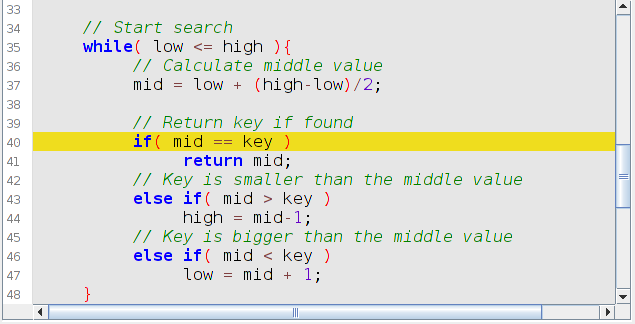
\includegraphics[width=0.7\textwidth]{./media/images/gui/main/CCompact-gui-left-code-2.png}
  \caption{Das Textfeld für den Sourcecode}
  \label{fig:gui-main-left-code}
\end{figure}

Die Zeile, in der sich der Cursor befindet, wird durch einen farbigen Balken markiert. Dieser Balken hat, je nach Modus des Debuggers, die selbe Farbe wie das Zustandspanel (siehe Abbildung \ref{fig:gui-main-left-code}).

Dieses Textfeld wird mit der statischen Methode \textbf{initCodePane()} der Klasse \textbf{InitLeftPanel} initialisiert. Die Methode wird beim Erstellen des linken Teils der Benutzeroberfläche aufgerufen.

\subsection{Ein- und Ausgabetextfeld}
\label{sec:gui-main-left-io}

Im Eingabefeld werden Daten eingegeben, die eingelesen werden, während der Debugger das Programm des Benutzers ausführt. Jedes Zeichen kann nur einmal eingelesen werden; bereits eingelesene Zeichen werden gelb hinterlegt (Abbildung \ref{fig:gui-main-left-io}). Die Ausgabedaten werden in einem separaten Textfeld dargestellt.

\begin{figure}[h!] 
  \centering
     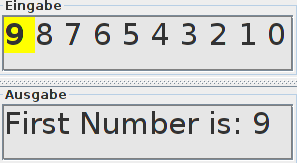
\includegraphics[width=0.4\textwidth]{./media/images/gui/main/io.png}
  \caption{Eingabedaten werden eingelesen, Ausgabe im Textfeld darunter}
  \label{fig:gui-main-left-io}
\end{figure}

In C Compact gibt es für Ein- und Ausgabe keine Konsole, wie sie bei einfachen Programmen meist verwendet wird. Bei unseren Versuchen (siehe Kapitel \ref{sec:sci-trial-intro}) hat sich gezeigt, dass dies die Schülerinnen und Schüler kaum stört. Besonders beim Entwickeln eines Algorithmus ist diese Methode der Ein- und Ausgabe besonders hilfreich, da die Eingabedaten nicht immer wieder eingegeben werden müssen.

Dem Interpreter muss immer ein Objekt, welches das Interface \textbf{StdInOut} (siehe Kapitel \ref{sec:deb-impl-interfaces}) aus dem Package \textbf{at.jku.ssw.cmm.debugger} implementiert, übergeben werden. In diesem Interface befinden sich Methoden zur Ein- und Ausgabe. Diese Methoden werden vom Debugger aufgerufen, wenn im Programm Anweisungen zur Ein- oder Ausgabe vorkommen.

\begin{lstlisting}[language=JAVA]
public interface StdInOut {
	public char in() throws RunTimeException;
	public void out(char arg0);
}
\end{lstlisting}

Für den Debugger wurde die Ein- und Ausgabe in der Klasse \textbf{IOstream} im Package \textbf{at.jku.ssw.cmm.debugger} implementiert. Die (gekürzte) Programmierung sieht wie folgt aus:

\begin{lstlisting}[language=JAVA]
@Override
public char in() throws RunTimeException {

	char c;
	try {
		// Zeichen lesen und aus der Liste löschen
		c = this.inputStream.get(0);
		this.inputStream.remove(0);
	} catch (Exception e) {
		// Throw interpreter runtime error if no more input data available
		throw new RunTimeException("no input data", null, 0);
	}
	
	// Gelesenes Zeichen im Textfeld markieren
	this.main.getLeftPanel().increaseInputHighlighter();
	
	return c;
}

@Override
public void out(final char arg0) {

	java.awt.EventQueue.invokeLater(new Runnable() {
		public void run() {
			// Zeichen zur Ausgabe hinzufügen
			main.getLeftPanel().outputStream("" + arg0);
		}
	});
}
\end{lstlisting}

Da der Interpreter in einem separaten Thread ausgeführt wird, muss die Ausgabe der übergebenen Daten in den \textbf{Event Dispatcher Thread} eingereiht werden. Für die Eingabedaten ist das nicht notwendig, da der Eingabestring in in einem Feld dieser Klasse gespeichert wird und als \textbf{final} deklariert wurde (siehe Kapitel \ref{sec:deb-impl-thread-problems}).

Für das Textfeld für die Eingabedaten wurde die Klasse \textbf{JInputDataPane} erstellt. Diese Klasse erbt von \textbf{JTextPane}\footnote{http://docs.oracle.com/javase/7/docs/api/javax/swing/JTextPane.html}. Die Klasse JInputDataPane ist im Package \textbf{at.jku.ssw.cmm.gui.init} zu finden. 

Die Textfelder werden mit den statischen Methoden \textbf{initInputPane()} und \textbf{initOutputPane()} der Klasse \textbf{InitLeftPanel} initialisiert.

\section{Rechter Teil der Benutzeroberfläche}
Der rechte Teil der Benutzeroberfläche besteht aus einem Zustandspanel für die aktuelle Aufgabe (Quest) und einem Panel mit mehreren Registerkarten, die unterschiedliche Bedienelemente enthalten, zum Beispiel für den Debugger (siehe Tabelle \ref{tab:gui-main-right-reg}).

Ähnlich wie der linke Teil der Benutzeroberfläche wird auch dieser Bereich von einer eigenen Klasse verwaltet. Die Klasse \textbf{GUIrightPanel} im Package \textbf{at.jku.ssw.cmm.gui} bildet eine Schnittstelle zwischen dem Hauptteil der Benutzeroberfläche (der Klasse \textbf{GUImain}, siehe Kapitel \ref{sec:gui-main-1}) und den Komponenten, die in den Registerkarten des rechten Panels eingebettet sind.

Wie bei der Klasse \textbf{GUIleftPanel} wird die Benutzeroberfläche dieses Bereiches mit der Methode \textbf{init} erstellt. Als Parameter wird eine Referenz auf \textbf{GUImain} übergeben, der Rückgabewert ist das fertig initialisierte rechte Panel.

\def\arraystretch{1.6}
\begin{table}[h!]
\begin{tabular}{|l|p{2.5cm}|p{6.6cm}|l|}
\hline
\textbf{Name}&\textbf{Sichtbar}&\textbf{Beschreibung}&\textbf{Siehe Kapitel}\\
\hline
Debug&Immer&Enthält Elemente zum Bedienen des Debuggers&\ref{sec:deb-use}\\
Error&Fehler aufgetreten&Zeigt detaillierte Informationen zu einem Fehler an&\ref{sec:deb-error}\\
Quest&Questsystem aktiv&Zeigt die aktuelle Aufgabenstellung an und ermöglicht das Überprüfen der Aufgabe&\ref{sec:quest}\\
Profile&Questsystem aktiv&Zeigt das Profil des Benutzers: Benutzerbild, Name und Auszeichnungen&\ref{sec:gui-main-right-questpanel}\\
\hline
\end{tabular}
\caption{Registerkarten im rechten Teil des Hauptfensters}\label{tab:gui-main-right-reg}
\end{table}

\subsection{Zustandspanel des Questsystems}
Dieses Zustandspanel visualisiert den aktuellen Status des Questsystems (siehe Kapitel \ref{sec:quest}) und ist daher auch nur gemeinsam mit diesem verfügbar (in Kapitel \ref{sec:gui-main-impl} wurde dargelegt, wie C Compact ohne den Funktionen des Questsystems gestartet werden kann). Die Zustände des Questsystems sind vollkommen unabhängig von denen des Debuggers.

Folgende Zustände können angezeigt werden:
\begin{enumerate}
\item \textbf{Keine Quest ausgewählt (Idle):} Zu Beginn hat der Benutzer noch keine Aufgabe ausgewählt, das Zustandspanel ist grau.
\item \textbf{Quest wird bearbeitet:} Während der Benutzer eine ausgewählte Aufgabe bearbeitet, ist das Panel blau.
\item \textbf{Quest wird getestet:} Wenn der Benutzer überprüfen will, ob er eine Aufgabe richtig erfüllt hat, startet er einen Test. Während des Tests wird das Zustandspanel gelb, im Regelfall ist dieser Status aber sehr kurz. Wenn während des Tests ein Fehler auftritt (wie etwa eine Endlosschleife), kann der Test in diesem Zustand abgebrochen werden.
\item \textbf{Test erfolgreich:} Verläuft der Test erfolgreich, wird das Zustandspanel grün.
\item \textbf{Test fehlgeschlagen:} In diesem Fall ist entweder ein Fehler im Sourcecode des Benutzers erkannt worden (eine detaillierte Beschreibung wird im Fehlerpanel angezeigt, siehe Kapitel \ref{sec:deb-error}) oder das Programm des Benutzers erfüllt die gestellte Aufgabe nicht.
\end{enumerate}

Der angezeigte Zustand wird mit folgenden Methoden der Klasse \textbf{GUIrightPanel} initialisiert. Diese Methoden sind wirkungslos, wenn das Questsystem deaktiviert ist.
\begin{lstlisting}[language=JAVA]
public void setIdleMode();
public void setQuestMode(String title);  // Titel der Quest
public void setTestMode();
public void setSuccessMode();
public void setFailedMode();
\end{lstlisting}

\subsection{Registerkarte \glqq{}Debug\grqq{}}
\label{sec:gui-main-right-reg-deb}
Diese Registerkarte ist immer die erste in der Reihenfolge der Tabs und ist jederzeit verfügbar. Im oberen Teil befindet sich ein Panel mit Bedienelementen des Debuggers, darunter werden die Variablen im Programm des Benutzers während der Laufzeit des Interpreters dargestellt (siehe Kapitel \ref{sec:deb-idea}).

Eine Referenz auf das Panel in dieser Registerkarte wird von folgender Methode übergeben:
\begin{lstlisting}[language=JAVA]
public GUIdebugPanel getDebugPanel() {
	return this.debugPanel;
}
\end{lstlisting}

\subsection{Registerkarte \glqq{}Error\grqq{}}
\label{sec:gui-main-right-error}
Wenn beim Debuggen ein Fehler im Compiler, Präprozessor oder Interpreter auftritt, wird dieses Panel sichtbar. Fehler im Quelltext des Benutzers, die beim Überprüfen einer Quest bemerkt werden, werden ebenfalls hier angezeigt. Ist der Fehler behoben und wurde das Programm erfolgreich ausgeführt, verschwindet diese Registerkarte automatisch.

Mit folgender Methode werden Fehlernachrichten eingeblendet. Als Parameter wird die Fehlernachricht des Compiler, Präprozessor oder Interpreter übergeben. Der Rückgabewert ist der Name (Präfix und Postfix) des Fehlers, wie er im Zustandspanel des Debuggers angezeigt wird. Siehe dazu Kapitel \ref{sec:gui-main-left-zust}.
\begin{lstlisting}[language=JAVA]
public String[] showErrorPanel(String errorCode);
\end{lstlisting}

Eine detaillierte Beschreibung zu der Verwaltung von Fehlerdokumenten ist in Kapitel \ref{sec:deb-error} zu finden.

\subsection{Registerkarte \glqq{}Quest\grqq{}}
In dieser Registerkarte werden Informationen und Bedienelemente zum Ausführen einer Aufgabe des Questsystems (siehe Kapitel \ref{sec:quest}) angezeigt.

Eine Referenz auf das Panel in dieser Registerkarte wird von folgender Methode übergeben:
\begin{lstlisting}[language=JAVA]
public GUITestPanel getTestPanel(){
	return this.testPanel;
}
\end{lstlisting}

Anmerkung: Dieses Panel wird - vor allem im Quelltext von C Compact - auch als \glqq{}testPanel\grqq{} bezeichnet, da der Benutzer mit Elementen dieses Komponenten überprüfen kann, ob er die aktuelle Aufgabe richtig gelöst hat.

\subsection{Registerkarte \glqq{}Profile\grqq{}}
\label{sec:gui-main-right-questpanel}
Hier werden Informationen zum aktuellen Benutzerprofil angezeigt.

Eine Referenz auf das Panel in dieser Registerkarte wird von folgender Methode übergeben:
\begin{lstlisting}[language=JAVA]
public ProfilePanel2 getProfilePanel() {
	return this.questPanel;
}
\end{lstlisting}

\section{Profile}
Da der Fortschritt eines Benutzers irgendwo gespeichert werden muss und ein Benutzer vielleicht irgendwann mit den Quests von vorne beginnen möchte oder sich mehrere Personen einen Computer teilen, gibt es Benutzerprofile. Dort werden der Fortschritt der Aufgaben und die Erfolge eines Benutzers gespeichert.

\subsection{Konzept}
Ein Profil ist das dynamische Gegenstück zu dem \textbf{statisch} mit dem Programm verknüpften Questsystem. Während Quest-Packages im Ordner \textbf{packages}, welcher sich direkt beim Programm befindet, abgelegt werden müssen, kann das Profil überall gespeichert werden. Somit kann das Profil ohne Probleme auf einem USB-Stick mitgenommen werden und auf einem beliebigen Computer, wo die benötigten Quest-Packete installiert sind, wieder geöffnet werden.

Wenn ein Profil an einem Computer geöffnet wird, an dem im Profil verzeichnete Quests nicht vorhanden sind, werden diese einfach nicht angezeigt und in den Profildaten nicht verändert.

\subsection{Dateien eines Profils}
Das Herzstück des Profils befindet sich in der Datei \textbf{profile.c}p. Diese ist in XML codiert. Darin sind Benutzername und Bildpfad sowie Statusinformationen zu den Quests vermerkt. Sobald ein Profilbild gesetzt wird, wird dieses in den Profilordner kopiert und als \textbf{avatar."<png">} abgespeichert. Danach wird der neue Avatar in der \textbf{profile.cp} vermerkt.

\begin{lstlisting}[language=XML]
<profile>
	<name>TestProfil</name>
	<profileimage>avatar.jpeg</profileimage>
	<state id="finished">
		<quest>01 Simples Hello World</quest>
		<package>01 Einstieg</package>
		<date>16-03-2015:15:37:361</date>
		<filepath>/home/peda/Arbeitsfläche/einstieg1.cmm</filepath>
		<token>Icon_Craft.xml</token>
	</state>
	...
</profile>
\end{lstlisting}
Wenn im Profil ein Profilbild gespeichert wird, wird dieses zuerst in den Profilordner mit einem angepassten Bildtitel kopiert. Nun wird das alte Profilbild entfernt. Sobald dies geschehen ist, wird im Profil das neue Profilbild vermerkt. Somit können keine Fehler aufgrund der falschen Codierung des Namens auftreten.

Für Errungenschaften, welche beim Fertigstellen vom Quests erreicht werden, wird die Ordnerstruktur bis zum Tokens-Ordner im Profil angelegt. Somit können Auszeichnungen auch dann angezeigt werden, wenn die Quest, für die der Benutzer die Errungenschaft erhalten hat, nicht mehr verfügbar ist.

Zu den zugehörigen Quests werden auch die Pfade zu den Benutzerprogrammen gespeichert. Somit können angefangene Quests wieder fortgesetzt werden.

Falls C Compact geschlossen wird und gerade eine Quest in Bearbeitung ist, wird diese im Profil mit dem Status \textbf{open} gekennzeichnet. Aus diesem Grund werden beim erneuten Öffnen des Profils automatisch die zuletzt verwendete Quest und die zugehörige \textbf{.cmm} Datei geladen.

\subsection{Variablen in der profile.java}
\begin{lstlisting}[language=JAVA]
	private String name;				//Profilname				
	private String profileimage;		//profilbild
	private String current;				//derzeit geöffnetes File
	private String profilePath;			//Pfad zum Profil
	private Quest quest;				//aktuelle Quest

	private String packagesPath;		//"packages" Ordner
	private List<Quest> profileQuests;	//Liste aller Quests im Profil
\end{lstlisting}
Die hier gezeigten Variablen werden größtenteils von der \textbf{profile.cp} bestimmt. 


\section{Menüleiste}
\label{sec:gui-main-menu}
Menüs sind bei der Gestaltung einer Benutzeroberfläche nahezu unerlässlich. Eine Menüleiste, bzw. ein Menü erleichtert dem Benutzer die Orientierung, da alle Funktionen auf einen Blick zu finden sind. Die Menüleiste wird auch in den \emph{Common User Access}\footnote{http://de.wikipedia.org/wiki/Common\_User\_Access} Richtlinien für die Gestaltung von Benutzeroberflächen definiert; diese Standards wurden 1989 von der Firma IBM festgelegt. Sie sind mittlerweile weit verbreitet und wurden in einer Reihe von Systemen umgesetzt.

Die Menüleiste wird in der statischen Methode \textbf{initFileM()} in der Klasse \\ \textbf{at.jku.ssw.cmm.gui.init.InitMenuBar} angelegt. Die Tastaturkürzel - \emph{\glqq{}Keyboard Shortcuts\grqq{}} - zum Beispiel \emph{Strg + S} zum Speichern, werden ebenfalls hier definiert. Beim Verwenden eines Tastaturkürzels wird der Event Listener des zugehörigen Menüeintrages aufgerufen.

Initialisieren eines Menüeintrages:
\begin{lstlisting}[language=JAVA]
// Menüeintrag wird initialisiert
JMenuItem openMI = new JMenuItem(_("Open"));

// Menüeintrag wird zum Menü hinzugefügt
fileM.add(openMI);

// Mit dem Action Listener verknüpfen, sodass dieser beim Anklicken des Menüs aufgerufen wird
openMI.addActionListener(listener.openHandler);

// Mit dem Keyboard Shortcut verknüpfen
openMI.setAccelerator(KeyStroke.getKeyStroke(KeyEvent.VK_O, ActionEvent.CTRL_MASK));

// Eintrag zur MenuBarControl hinzufügen
menuBarControl.add(newMI);
\end{lstlisting}

Die Events der Menüleiste werden in der Klasse \textbf{MenuBarEventListener} im Paket \textbf{at.jku.ssw.cmm.gui.event} abgewickelt. Diese Klasse enthält Methoden, die bestimmte Aktionen ausführen und innere Klassen, die einen Event Listener implementieren und diese Methoden aufrufen. Diese Aufteilung ist nötig, da bestimmte Aktionen auch von anderen Instanzen aufgerufen werden können (zum Beispiel wird auch gespeichert, wenn der Benutzer C Compact schließt).

\subsection{Aktivieren und Deaktivieren von Menüeinträgen}
\label{sec:gui-main-menu-ctrl}
Da während der Debugger ausgeführt wird keine Aktionen erlaubt sind, die den Text im Sourcecode Textfeld ändern (siehe Kapitel \ref{sec:gui-main-left-code}), werden bestimmte Menüeinträge aktiviert oder deaktiviert, wenn sich der Status des Debuggers ändert (Siehe Kapitel \ref{sec:gui-main-left-zust}). Diese Aktionen werden in der Klasse \textbf{at.jku.ssw.cmm.gui.MenuBarControl} zusammengefasst. Diese Klasse enthält eine Liste, in der alle Menüeinträge referenziert werden, die beim Ausführen des Debuggers deaktiviert werden sollen. Mit der Methode \textbf{add()} werden Objekte in diese Liste eingetragen.
\begin{lstlisting}[language=JAVA]
public void add(JMenuItem mi){
	this.list.add(mi);
}
\end{lstlisting}

Mit den Methoden \textbf{lockAll()} und \textbf{unlockAll()} werden diese Menüeinträge dann deaktiviert oder aktiviert.

\begin{lstlisting}[language=JAVA]
public void lockAll();
public void unlockAll();
\end{lstlisting}

Des Weiteren kann in dieser Kontrollklasse ein Menüeintrag definiert werden, der eine Liste der zuletzt geöffneten Dateien enthält. Mit der Methode \textbf{setRecentMenu(...)} wird dieser Menüeintrag definiert:
\begin{lstlisting}[language=JAVA]
public void setRecentMenu( JMenu mi ){
	this.recentMI = mi;
}
\end{lstlisting}

Dieses Untermenü wird mit der Methode \textbf{updateRecentFiles(...)} aktualisiert.
\begin{lstlisting}[language=JAVA]
public void updateRecentFiles( List<String> recentFiles, String currentFile );
\end{lstlisting}

Im Untermenü \glqq{}Sourcecode\grqq{} (siehe Kapitel \ref{sec:gui-menu-code}) gibt es Funktionen zum Aufheben bzw. Wiederholen der letzten Aktion der Textbearbeitung (\emph{undo} und \emph{redo}). Diese Menüeinträge sollen aber nur aktiviert sein, wenn eine solche Aktion tatsächlich möglich ist. Beispielsweise kann nach dem Start des Programmes nichts rückgängig gemacht werden, da noch keine Aktionen durchgeführt wurden. Außerdem dürfen diese Aktionen nicht ausgeführt werden, wenn der Debugger gerade läuft, da der Sourcecode sonst während der Laufzeit verändert werden würde.

Referenzen auf die beiden entsprechenden Menüeinträge werden in der Klasse MenuBarControl separat gespeichert.
\begin{lstlisting}[language=JAVA]
public void setUndo(JMenuItem undo){
	this.undo = undo;
}

public void setRedo(JMenuItem redo){
	this.redo = redo;
}
\end{lstlisting}

Mit der Methode \textbf{updateUndoRedo(...)} werden die Zustände dieser Menüeinträge aktualisiert. Als Parameter werden eine Referenz auf das Textfeld mit dem Sourcecode und eine boolean-Variable übergeben. Letztere ist \textbf{true}, wenn der Debugger gerade läuft.
\begin{lstlisting}[language=JAVA]
public void updateUndoRedo( RSyntaxTextArea tArea, boolean running ){
	this.undo.setEnabled(!running & tArea.canUndo());
	this.redo.setEnabled(!running & tArea.canRedo());
}
\end{lstlisting}

\subsection{Menü \glqq{}Datei\grqq{}}
\label{sec:gui-main-menu-file}
Das wohl bekannteste Menü in jedem Programm ist das Menü \glqq{}Datei\grqq{}. In C Compact enthält es neben den grundlegenden Funktionen zum Öffnen oder Speichern einer vorhandenen oder neuen Datei auch noch weitere Funktionen. Der Eintrag \glqq{}Drucken\grqq{} verwendet eine Methode, die in der RSyntaxTextArea implementiert ist, allerdings treten bei der Formatierung oft Probleme auf. Wesentlich wichtiger sind die Menüpunkte \glqq{}Einstellungen\grqq{} (siehe Kapitel \ref{sec:win-set}), \glqq{}Sprache\grqq{} (siehe Kapitel \ref{sec:win-lang}) und \glqq{}Über C Compact\grqq{} (siehe Kapitel \ref{sec:win-credits}). Schließlich gibt es noch dem Menüpunkt \glqq{}Beenden\grqq{}, C Compact kann aber auch mit der Tastenkombination \emph{Alt + F4} (diese Kombination wird in den meisten Betriebssystemen und Oberflächen bereits standardmäßig verwendet) oder über entsprechende Bedienelemente im Fensterrahmen geschlossen werden.

\subsection{Menü \glqq{}Sourcecode\grqq{}}
\label{sec:gui-menu-code}
Dieses Menü würde in den meisten Programmen dem Menü \glqq{}Bearbeiten\grqq{} entsprechen. Allerdings beziehen sich die Menüeinträge wie \glqq{}Kopieren\grqq{}, \glqq{}Einfügen\grqq{}, \glqq{}Rückgängig\grqq{}, etc. immer auf das Textfeld für den Sourcecode --- mit dem Menünamen sollen also Verwechslungen vermieden werden --- und andererseits enthält dieses Menü auch Einträge zum Steuern des Debuggers. Diese Einträge sollen vom Benutzer kognitiv mit dem Sourcecode verknüpft werden.

\subsection{Menü \glqq{}Fortschritt\grqq{}}
Dieses Menü enthält Einträge, die das Questsystem (siehe Kapitel \ref{sec:quest}) betreffen. Mit \glqq{}Profil Wählen\grqq{} Wird C Compact beendet und der Launcher (siehe Kapitel \ref{sec:win-launcher}) gestartet, sodass der Benutzer ein anderes Profil wählen kann. Mit dem Befehl \glqq{}Profil Exportieren\grqq{} kann der Benutzer sein Profil an einem anderen Ort speichern (siehe Kapitel \ref{sec:quest-export}). Der Menüeintrag \glqq{}Quest wählen\grqq{} öffnet ein Fenster zum Auswählen eines Questpaketes; im Anschluss kann der Benutzer eine Aufgabe zum Bearbeiten wählen (siehe Kapitel \ref{sec:gui-elements-package-sel}). Mit \glqq{}Questpaket importieren\grqq{} kann ein Package importiert werden (siehe Kapitel \ref{sec:quest-import}).

